\chapter{Riconciliazione sorgenti}

Nel seguito verranno documentati i passi intrapresi nella progettazione
del modello riconciliato o Operational Data Store partendo dalle sorgenti
operazionali descritte nel capitolo precedente.

\section{Ispezione e normalizzazione}

\subsection{Helbiz}

Il livello di granularità delle profilazioni della sorgente Helbiz è
risultato essere troppo basso rispetto alle interrogazioni a cui il data
warehouse si prefigge di rispondere. Inoltre attributi come
\textit{latitude}, \textit{longitude}, \textit{battery\_level\_miles},
\textit{power} e \textit{miles\_range} non si prestano, in quanto valori
numerici continui, ad essere utilizzati all'interno del costrutto di
selezione di una interrogazione OLAP per il dominio applicativo
scelto. Inoltre gli attributi \textit{battery\_level\_miles} e
\textit{miles} risultano essere ridondanti.

Partendo dallo schema ER mostrato in figura~\ref{fig:vehicle_profiling_er} è
stato ricavato lo schema concettuale di figura
\ref{fig:vehicle_interval_profiling_er}.

\begin{figure}[H]                                                                                                                                                            
\centering                                                                                                                                                                   
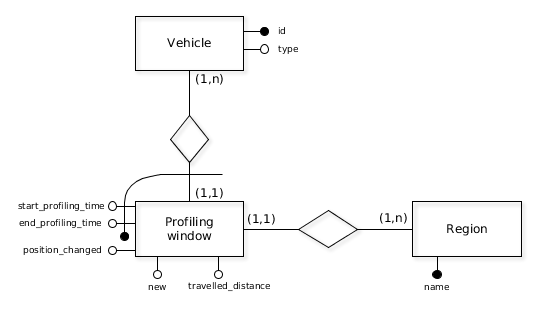
\includegraphics[width=\textwidth]{diagrams/vehicle_interval_profiling_er}                                                                                                                                   
\caption{Diagramma ER Vehicle-Profiling window-Region}                                                                                                                                            
\label{fig:vehicle_interval_profiling_er}                                                                                                                                                           
\end{figure}

Non essendo il nuovo schema una semplice ristrutturazione dello
schema logico di partenza ma un nuovo schema a se stante, l'entità
\textit{Profiling} è stata sostituita con l'entità \textit{Profiling
window}, le cui istanze si riferiscono ai dati profilati all'interno di
un delimitato intervallo di tempo per un determinato veicolo.
Nello specifico sono stati aggiunti i seguenti nuovi attributi:
\begin{itemize}
\item \textit{start\_profiling\_time:} istante di inizio della finestra
temporale;
\item \textit{end\_profiling\_time:} istante di fine della finestra temporale;
\item \textit{position\_changed:} attributo che indica se la posizione
del veicolo è variata durante l'intervallo in oggetto;
\item \textit{new:} attributo che indica se un veicolo non presente durante
all'istante di inizio della finestra temporale è stato invece censito
all'istante che delimita la fine della finestra temporale;
\item \textit{travelled\_distance:} attributo che contiene la distanza 
percorsa dal veicolo nella finestra temporale.
\end{itemize}

\noindent~L'attributo \textit{travelled\_distance} corrisponde alla distanza in linea
d'aria tra le coordinate cartesiane della profilazione effettuata all'istante
\textit{start\_profiling\_time} e quella effettuata all'istante
\textit{end\_profiling\_time}.
L'aggiunta dell'attributo \textit{new} è volta a gestire il caso in cui un
veicolo sia stato oggetto di utilizzo ininterrotto da parte di un utente per
un tempo superiore all'intervallo tra due successive profilazioni o il caso in
cui un veicolo sia stato intenzionalmente posizionato in un punto da un addetto
della manutenzione di Helbiz dopo essere stato ricaricato o allo scopo di
redistribuzione la flotta di veicoli a disposizione all'interno della region.
L'attributo \textit{position\_changed} è stato aggiunto allo scopo di permettere
una veloce selezione delle istanze dell'entità in oggetto per le quali lo
spostamento memorizzato nell'attributo \textit{travelled\_distance} risulta essere
maggiore una certa soglia. Come sarà descritto nella parte dedicata alle attività di
ETL eseguite dalle sorgenti operazionali all'ODS, tale attributo permette di
escludere una serie di falsi positivi dati dalla presenza dei veicoli in ambienti
aperti, soggetti agli eventi atmosferici oltre che all'interazione con attori
che si trovano nelle immediate vicinanze.
Inoltre si ha che gli attributi \textit{start\_profiling\_time} e
\textit{end\_profiling\_time} insieme con l'attributo \textit{id} dell'entità
\textit{Vehicle}, identificano univocamente una finestra di profilazione.

Anche quest'ultimo schema risulta lontano dal poter essere integrato con le altre
sorgenti, aventi un livello di granularità temporale minimo di un ora.
Inoltre gli attributi \textit{position\_changed} e \textit{new} non sono
sfruttabili in nessuna delle interrogazione derivate dal fatto definito.
Pertanto, partendo dallo schema concettuale di
figura~\ref{fig:vehicle_interval_profiling_er} si è giunti allo schema di figura
\ref{fig:vehicle_hour_profiling_er}.

\begin{figure}[H]                                                                                                                                                            
\centering                                                                                                                                                                   
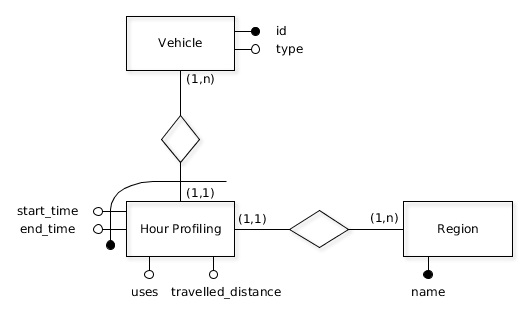
\includegraphics[width=\textwidth]{diagrams/vehicle_hour_profiling_er}                                                                                                                                   
\caption{Diagramma ER Vehicle-Profiling window-Region}                                                                                                                                            
\label{fig:vehicle_hour_profiling_er}                                                                                                                                                           
\end{figure}

Il processo di ristrutturazione ha consistito nella sostituzione dell'entità
\textit{Profiling window} con l'entità \textit{Hourly Profiling} avente i
seguenti nuovi attributi:
\begin{itemize}
\item \textit{start\_time:} istanze d'inizio della finestra di profilazione;
\item \textit{end\_time:} istanze di fine della finestra di profilazione;
\item \textit{uses:} attributo contenente il numero di utilizzi di un
veicolo all'interno della finestra di profilazione;
\item \textit{travelled\_distance:} attributo che contiene la distanza 
percorsa dal veicolo nella finestra di profilazione.
\end{itemize}
Tale schema è pertanto da considerarsi quale schema concettuale definitivo per la
sorgente Helbiz e come uno degli schemi oggetto del successivo processo di
integrazione.

\subsection{Torino Meteo}

Similmente a quanto fatto per Helbiz, anche per la sorgente Torino Meteo è
stato necessario modificare lo schema concettuale presentato in figura
\ref{fig:weather_detection_er}. Le profilazioni acquisite dai sensori
sono relative ad un determinato istante di tempo e non ad una finestra temporale
come nel caso di Helbiz e riportano per gli attributi \textit{rain},
\textit{wind}, \textit{relative\_humidity} e \textit{temperature} valori numerici
continui che non si prestano ad essere utilizzati all'interno di un'interrogazione
OLAP quali quelle definite. Inoltre, gli attributi \textit{id} e
\textit{relative\_humidity} non sono di interesse ai fini del progetto.
Lo schema derivato di figura \ref{fig:wheathre_hourly_profiling_er} contiene la
nuova entità \textit{Weather hourly profiling} caratterizzata dai seguenti attributi:
\begin{itemize}
\item \textit{start\_profiling\_time:} istante di inizio dell'intervallo orario in cui
si collocano l'entità in oggetto;
\item \textit{end\_profiling\_time:} ora di fine dell'intervallo orario in cui si
collocano le profilazioni rappresentate dall'entità in oggetto;
\item \textit{rain\_level:} attributo contenente il livello di intensità delle
precipitazioni rilevato nell'intervallo orario;
\item \textit{wind\_level:} attributo contenente il livello di intensità del
vento rilevato nell'intervallo orario;
\item \textit{temperature\_level:} attributo contenente il livello di intensità della
temperatura rilavato nell'intervallo orario.
\end{itemize}

\begin{figure}[H]                                                                                                                                                            
\centering                                                                                                                                                                   
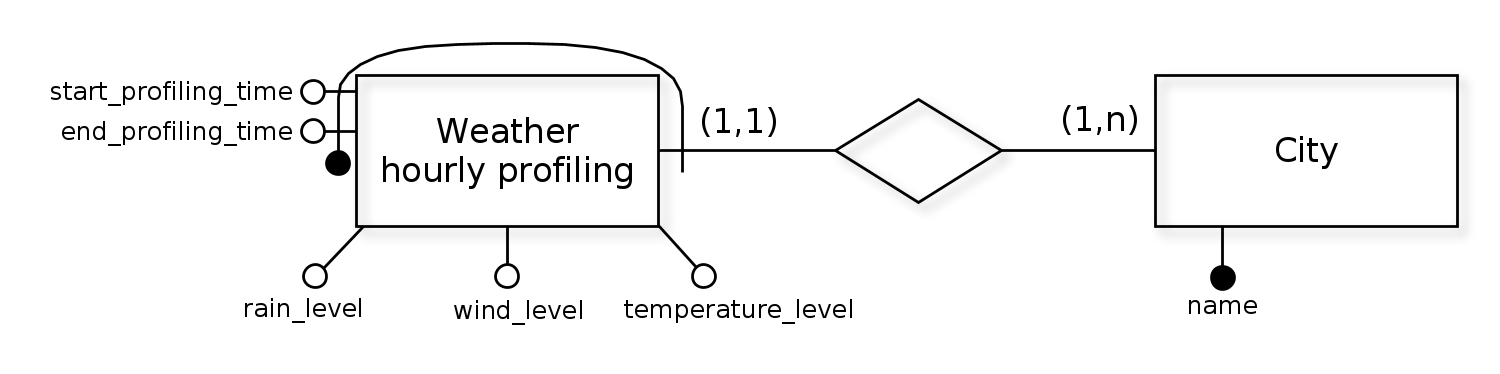
\includegraphics[width=\textwidth]{diagrams/wheathre_hourly_profiling_er}                                                                                                                                   
\caption{Diagramma ER Vehicle-Profiling window-Region}                                                                                                                                            
\label{fig:wheathre_hourly_profiling_er}                                                                                                                                                           
\end{figure}

Lo schema precedentemente descritto è da considerarsi quale schema concettuale definitivo
per la sorgente Torino Meteo e come uno degli schemi partecipanti al successivo processo di
integrazione.

\subsection{Scioperi}

Per la sorgente Scioperi non è stato necessario procedere ad alcuna ristrutturazione dello
schema concettuale di figura~\ref{fig:strikes_er} che sarà pertanto insieme ai precedenti
oggetto della successivo processo di integrazione.

\section{Integrazione}

\subsection{Preintegrazione}

Essendo i dati relativi ad ogni sorgente operazionale considerata ottenuti
attraverso l'interrogazione di una API, solo un sottoinsieme tra entità,
relazioni e attributi rilevanti ai fini del progetto sono stati considerati
al momento della redazione dei precedenti schemi concettuali. Non è stato
quindi necessario escludere alcuna parte dei dati dall'integrazione. 

La semplicità dei diagrammi concettuali di ognuna delle tre sorgenti ha
permesso di utilizzare una strategia di integrazione ennaria single step.

\subsection{Comparazione e allineamento schemi}

\subsubsection{Conflitti sui nomi}

Si evidenzia tra lo schema concettuale della sorgente Helbiz e quello della
sorgente Torino Meteo una sinonimia rispettivamente tra i nomi delle
relazioni \textit{Region} e \textit{City}. Le stesse vengono risolte nello
schema concettuale integrato utilizzando il nome \textit{City} per l'entità
in questione.

\subsubsection{Conflitti strutturali}
E' presente un conflitto strutturale relativo alla diversa rappresentazione 
dell'entità città, per le sorgenti Helbiz e Torino Meteo come entità,
per la sorgente Scioperi come attributo dell'entità \textit{Strike}.
Si risolve tale conflitto adottando la rappresentazione come entità
come gestito negli schemi concettuali della altre due sorgenti.

\subsection{Fusione e ristrutturazione schemi}

Il risultato della sovrapposizione degli schemi e delle scelte intraprese nella
risoluzione dei conflitti ha portato allo schema di figura~\ref{fig:integrated_1_er}.

\begin{figure}[H]                                                                                                                                                            
\centering                                                                                                                                                                   
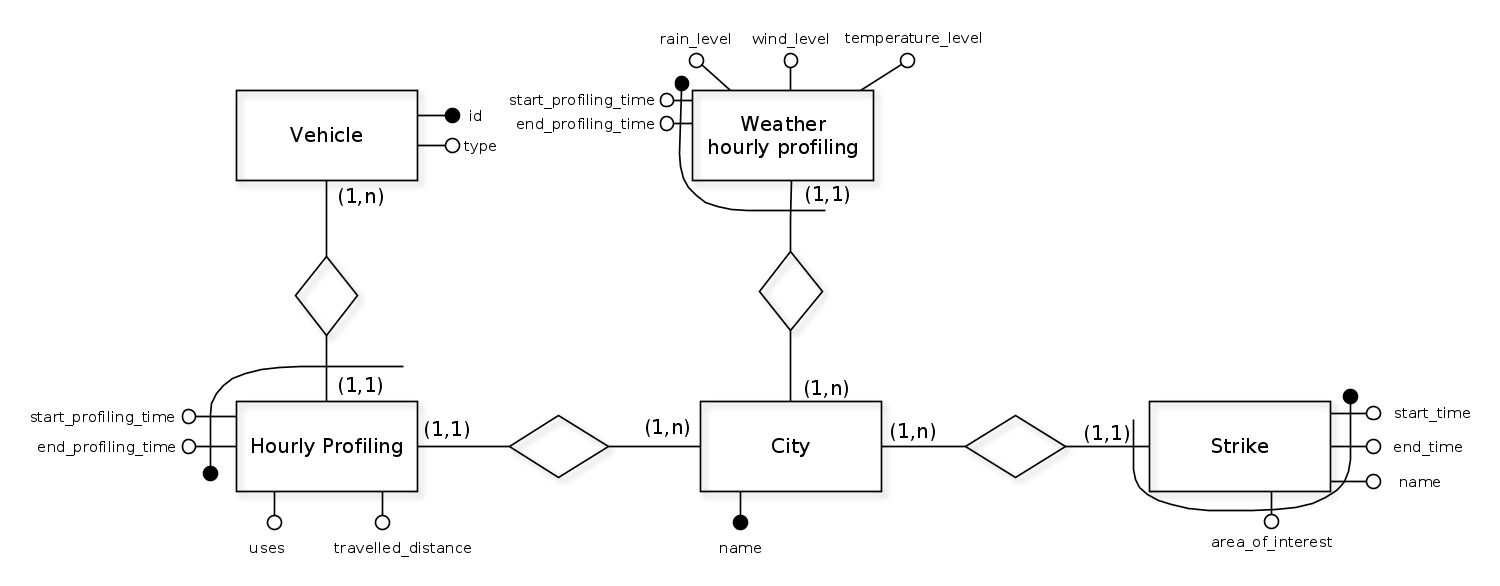
\includegraphics[width=\textwidth]{diagrams/integrated_1_er}                                                                                                                                   
\caption{Diagramma ER Vehicle-Profiling window-Region}                                                                                                                                            
\label{fig:integrated_1_er}                                                                                                                                                           
\end{figure}

In figura~\ref{fig:riconciliato_er} è mostrato lo schema logico dell'ODS.
Alla tabella \textit{cities} è stato aggiunta una chiave surrogata \textit{id}
verso la quale vi è un vincolo di integrità referenziale per ognuna delle tabelle
ad essa relazionate. Tale attributo è poi parte della chiave primaria per le
tabelle \textit{strikes} e \textit{weather\_hourly\_profilings}.

Diversamente da quanto fatto in fase di progettazione dello schema logico della
sorgente operazionale, si è scelto di rappresentare le entità \textit{Vehicle}
e \textit{Vehicles\_hourly\_profilings} con due le relazioni eliminando la
ridondanza dell'attributo \textit{type}. 

Si noti inoltre la presenza dell'attributo \textit{insert\_time} per la
tabella \textit{cities}, verrà fatto riferimento allo stesso nelle due procedure
di ETL; nello specifico esso sarà popolato durante la fase di popolamento
dell'ODS e sarà letto nella fase di popolamento dei data mart.

\begin{figure}[H]                                                                                                                                                            
\centering                                                                                                                                                                   
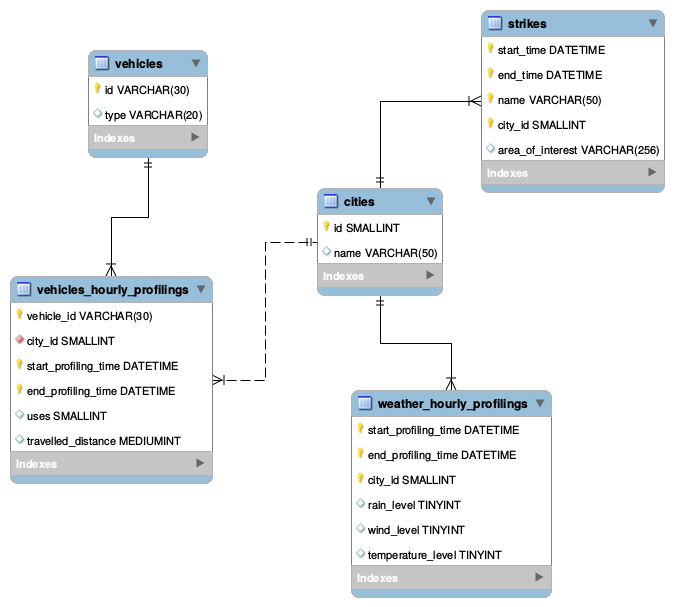
\includegraphics[width=\textwidth]{diagrams/riconciliato_er}                                                                                                                                   
\caption{Schema Riconciliato - Diagramma logico}                                                                                                                                            
\label{fig:riconciliato_er}                                                                                                                                                           
\end{figure}

\label{sec:etl_sorgenti_ODS}
\section{ETL da sorgenti operazionali a ODS}

\subsection{Helbiz}

\subsubsection{Estrazione}

La sorgente dati per sua natura di tipo transiente (i dati sono disponibili in
real-time e non sono disponibili dati storici) è stata trasformata in una
sorgente con dati periodici in quanto si è scelto di conservare i dati raccolti
mediante le API per un periodo di 6 mesi.

L'estrazione è di tipo \textit{incremental delayed}: un job di sistema è
schedulato al termine della giornata per invocare l'applicativo sviluppato in
modalità di estrazione il quale interroga la base dati, ottenere i dati delle
profilazioni delle ultime 24 ore e procedere al caricamento delle stesse
all'interno dell'ODS.

\subsubsection{Trasformazione}

Durante la procedura di estrazione viene interrogata la tabella
\textit{vehicles} dello schema di figura~\ref{fig:vehicles_logic_physic} al fine
di ottenere tutti gli istanti di profilazione intervenuti nelle ultime 24 ore
per una determinata region, ordinati in maniera ascendente. Viene eseguita
a livello di codice Java la differenza tra coppie adiacenti di
\textit{query\_time} e vengono scartate le coppie per cui la differenza in
minuti non è compresa tra 3 e 10 minuti intervalli esclusi. Come anticipato
l'applicativo è stato impostato per acquisire dati dal servizio remoto ogni 5
minuti. Applicando tale operazione di filtraggio si ha la sicurezza di evitare
di processare profilazioni tra loro troppo vicine o troppo distanti, frutto in
qualche caso di errore dovuto alla momentanea incapacità di rispondere da parte
del servizio remoto. Per ogni coppia di istanti di misurazione viene effettuata
un'interrogazione al database della sorgente al fine di ottenere per ogni veicolo
della region di interesse una tupla ricavata dalla join della tabella
\textit{vehicles} con se stessa avendo cura di associare coppie di profilazioni
aventi stesso id, stessa città e diversa \textit{query\_time} preso dalla coppia
ottenuta. A questo punto, per ogni coppia vengono prese latitudine e longitudine,
convertite in radianti e viene calcolata la distanza in linea d'aria espressa in
metri mediante l'uso delle seguenti tre formule:

\begin{gather}
\varphi = \abs{\mathit{lon}_1 - \mathit{lon}_2}, \notag \\
\Delta = \arccos(\sin(\mathit{lat}_2) \cdot \sin(\mathit{lat}_1) + \cos{\mathit{lat}_2} \cdot \cos(\mathit{lat}_1) \cdot \cos(\varphi)), \notag \\
\mathit{d} = \Delta \cdot 6371000. \notag
\end{gather}

\noindent~Nello specifico, nell'ultima formula è utilizzato il raggio della
terra per calcolare la distanza tra i due punti. La distanza ottenuta è
confrontata con una soglia fissata a 100 metri. Se la distanza in linea d'aria
è superiore a tale valore, allora è possibile considerare che il veicolo in
questione stato utilizzato nell'intervallo considerato. Tale soglia serve
ad escludere errori nella segnalazione della posizione o spostamenti causati da
attori esterni non allo scopo di utilizzare il veicolo per spostarsi 
non rilevanti allo scopo del progetto (\textit{e.g.} i veicoli possono essere spostati con un automezzo causa manutenzione o per operazioni stoccaggio). 
Quanto ottenuto da ogni coppia di veicoli è via via inserito in una query di INSERT che provvede ad inserire i risultati
nella tabella \textit{vehicles\_profilings} di figura~\ref{fig:ETL_veicoli_er}.
La colonna \textit{position\_changed} contiene un valore booleano sulla base
del prevedente confronto eseguito sulla distanza in linea d'aria calcolata.
Al termine del processamento di tutte le coppie per un determinato intervallo,
viene eseguita un'altra query sulla tabella \textit{vehicles} della sorgente allo 
scopo di estrarre i veicoli rilevati nella misurazione più recente e non nella  
misurazione temporalmente precedente. In tal modo è possibile tenere conto dei
veicoli che in quanto utilizzati o disattivati non erano disponibili al momento 
della prima interrogazione ma lo sono diventati al momento della seconda. Per 
ognuno dei veicoli risultato di tale query è aggiunto un record alla tabella
\textit{vehicles\_profilings} avente valore nullo per le colonne 
\textit{position\_changed} e \textit{travelled\_distance} e avranno valore
1 per la colonna booleana \textit{new}. La tabella \textit{vehicles\_profilings}
ha funzione di buffer per le successive operazioni di \textit{enrichment} e risiede
nell'ODS.

Al termine del processamento delle coppie di rilevazioni viene interrogata la tabella
appena riempita e vengono estratti tutti i record delle rilevazioni aventi come
\textit{start\_profiling\_time} un valore compreso nelle 24 ore precedenti.
Per ogni record estratto sono eseguite a livello di codice Java le seguenti
operazioni:
\begin{itemize}
\item l'attributo \textit{start\_profiling\_time} di tipo \java{DATETIME} viene
ricondotto all'inizio dell'ora ricavando così un'ora d'inizio;
\item viene verificata in una struttura dati di tipo \java{Map} allocata in
memoria la presenza di un valore passando come chiave l'attributo \textit{id}
del veicolo oggetto della profilazione; se presente il valore ritornato consiste un
oggetto di tipo \java{Map} che associa ad ogni ora di un giorno una mappa,
quest'ultima contenente le chiavi \textit{uses} e \textit{travelled\_distance}
ed i relativi valori numerici associati; in caso non esiste un oggetto associato
all'ora passata come chiave, tale mappa viene creata ed le vengono associato
valore 0 per ognuno dei precedenti attributi;
\item se l'attributo \textit{position\_changed} è settato a 1 e la distanza
\textit{travelled\_distance} è inferiore a 3000 metri, l'algoritmo procede
ad incrementare la entry con chiave \textit{uses} e ad aggiungere la distanza
percorsa all'attributo \textit{travelled\_distance}; considerando che i veicoli
in esame hanno una velocità massima di 25\,km/h, e da ciò che la massima distanza
percorribile in un tempo di 5 minuti è di 2\,km, la cifra limite utilizzata nel
precedente confronto è stata ottenuta moltiplicando per 1,5 tale distanza;
\item se l'attributo \textit{new} è invece settato a 1, viene eseguito
un controllo tra le profilazioni aventi \textit{end\_profiling\_time} eguale
alla \textit{start\_profiling\_time} corrente e, nel caso in cui tale veicolo
risulti presente in tale finestra di profilazione antecedente a quella in oggetto
se ne calcola la distanza percorsa con l'utilizzo delle formule mostrate in
precedenza; nel caso in cui la distanza risulti realisticamente percorribile
nel corso di 10 minuti di tempo, allora si procede con le stesse modalità
del punto precedente all'incremento degli attributi \textit{uses} e
\textit{travelled\_distance}.
\end{itemize}
I dati contenuti nella mappa presente in memoria vengono inseriti nella
tabella \textit{vehicles\_hourly\_profilings}, appartenente anch'essa all'ODS
ed oggetto del processo di integrazione precedente.

Ogni region ha come attributo un nome sotto forma di stringa alfanumerica
minuscola. E' però necessario convertire tale stringa nel nome
della corrispondente città, valore utilizzato dalle altre due sorgenti
oggetto dell'integrazione. Entra quindi in gioco una procedura di
\textit{cleansing} che utilizzando una tabella di supporto, provvede a
modificar il valore dell'attributo \textit{city\_id} della tabella
\textit{vehciles\_profilings} con l'id della corrispondente città della
tabella \textit{cities} dell'ODS, il tutto mediante una query di UPDATE
la quale esegue una JOIN su di una tabella di traduzione appositamente
definita.

Con tale operazione termina la procedura di trasformazione dei dati.
In figura~\ref{fig:ETL_veicoli_er} è mostrato lo schema logico della due tabelle
oggetto della procedura di trasformazione qui descritta e della tabella
\textit{cities} ad esse associata.

\subsubsection{Caricamento}

La procedura di caricamento è di tipo incrementale, consiste nella sola aggiunta di
nuovi record alla tabella e viene eseguita con cadenza giornaliera, al termine della
procedura di trasformazione. Il tutto è svolto dall'applicativo Java sviluppato che
si occupa nell'ordine di:
\begin{itemize}
\item inserire nella tabella \textit{vehicles} i record relativi a veicoli non ancora
inseriti che sono stati oggetto di profilazioni durante la giornata precedente;
\item inserire nella tabella \textit{cities} i record relativi a nuove città oggetto
di profilazione durante la giornata precedente;
\item estrarre i dati dalla tabella \textit{cities} della sorgente e utilizzare la
tabella di traduzione al fine di verificare la presenza della versione tradotta della
stessa all'interno dell'ODS e in caso contrario procedere all'aggiunta;
\item estrarre dal database delle sorgente i record inseriti durante la precedente
giornata (per i quali l'attributo \textit{query\_time} si riferisce ad un istante che
si colloca nelle precedenti 24 ore) comprensivi dell'attributo \textit{name} della
tabella \textit{city};
\item procedere all'inserimento dei record ottenuti al punto precedente ottenendo
per ogni valore dell'attributo \textit{cities.name}, per mezzo del costrutto JOIN,
il \textit{city\_id} corrispondente della tabella \textit{cities} dell'ODS, al fine
di mantenere l'integrità referenziale.
\end{itemize}

\subsection{Torinometeo}

\subsubsection{Estrazione}

Si ha a che fare con una sorgente con dati periodici per la quale si è scelto di 
conservare dati per i successivi 6 mesi a partire dalla raccolta degli stessi.

L'estrazione è di tipo \textit{incremental delayed}: un job di sistema è
schedulato al termine della giornata per invocare l'applicativo sviluppato in
modalità di estrazione il quale interroga la base dati, ottiene i dati
memorizzati nelle ultime 24 ore e procedere al caricamento degli stessi
all'interno dell'ODS.

\subsubsection{Trasformazione}

Come anticipato, i dati raccolti nel database della sorgente sono relativi a
misurazioni realizzate dal sensore nell'istante in cui quest'ultimo viene
interrogato. Tali dati non si prestano ad essere associati alle rilevazioni
sull'utilizzo orario dei veicoli. Segue una procedura di enrichment la quale
provvede nell'ordine a:
\begin{itemize}
\item trasformare il valore di tipo \java{DATETIME} dell'attributo
\textit{query\_time} nell'ora esatta precedente più prossima (operazione
equivalente a porre ad azzerare minuti e secondi);
\item eseguire la media delle somme degli attributi \textit{wind\_level},
\textit{temperature\_level} e \textit{rain\_level} di tutti i record per i
quali l'attributo \textit{query\_time} rappresenta lo stesso istante o un
istante più recente, distante meno di un'ora dalla data calcolata al punto
precedente;
\item confrontare per ognuno degli attributi calcolati la relativa tabella
dei livelli la quale associa un valore da 0 a 4 sulla base dell'appartenenza
o meno al range di valori associato al livello corrispondente; in tal modo si
rendono discreti i valori di tali attributi e quindi candidati ad essere 
oggetto di interrogazione;
\item creare un record da inserire nella tabella
\textit{weather\_hourly\_profilings} a partire dai dati ottenuti ai punti
precedenti; nello specifico, per l'attributo
\textit{start\_profiling\_time} viene presa la data calcolata al primo punto;
a tale data è sommata un ora per ottenere il valore dell'attributo
\textit{end\_profiling\_time}; ad ognuno degli attributi relativi alle
condizioni atmosferiche è associato il livello ottenuto al punto precedente;
l'attributo \textit{city\_id} è invece ottenuto per mezzo di una JOIN tra il
nome della città estratta dalla base dati della sorgente e la tabella
\textit{cities} dell'ODS.
\end{itemize}
Tali passi sono ripetuti per ogni ora della precedente giornata.

Le operazioni precedenti, eseguite interamente attraverso l'esecuzione di script
SQL, sono eseguite dall'applicativo Java scritto al termine della precedente
procedura di estrazione.

\subsubsection{Caricamento}

Il caricamento è di tipo incrementale e consiste nella sola aggiunta dei nuovi
record alla tabella \textit{weather\-hourly\_profilings} e avviene con cadenza
giornaliera al termine della precedente procedura di trasformazione.
L'applicativo Java preposto si occupa di:
\begin{itemize}
\item inserire nella tabella \textit{cities} i record relativi a nuove città oggetto
di profilazione durante la giornata precedente;
\item procedere all'inserimento dei record risultanti dalla precedente procedura di
trasformazione facendo in modo di inserire per l'attributo \textit{city\_id}
la corrispondente chiave della tabella \textit{cities} dell'ODS, al fine
di mantenere l'integrità referenziale.
\end{itemize}

\subsection{Scioperi}

\subsubsection{Estrazione}

Si ha a che fare con una sorgente con dati periodici per la quale si è scelto di 
conservare dati per i successivi 6 mesi a partire dalla raccolta degli stessi.

Come per le precedenti due sorgenti l'estrazione è di tipo
\textit{incremental\_delayed} ed è effettuato con le stesse modalità di estrazione
utilizzate per le precedenti sorgenti. E' invece presente una differenza sui dati
memorizzati che si riferiscono a scioperi avvenuti non meno di due giorni prima
della data corrente. Come anticipato al momento della descrizione della sorgente,
tali open data hanno anche funzionalità di forecasting ricomprendendo tra gli scioperi
anche quelli previsti nel futuro ed annunciati. Gli scioperi, compresi quelli in corso,
sono soggetti anche a modifiche ed annullamenti. Considerato che il dato sulla
presenza o meno di uno sciopero è da ritenersi attendibile alla fine dello
sciopero stesso, si è scelto di inserire ad ogni aggiornamento della base dati
della sorgente i dati sui soli scioperi aventi data precedente di due giorni la
data corrente al fine di gestire anche il caso di scioperi della durata superiore 
ad un giorno.

Inoltre, al fine di ottimizzare il processo di estrazione, nell'interrogazione
vengono selezionati i record degli scioperi relativi alle sole città di interesse,
ovvero quelle presente nella base dati della sorgente Helbiz.

\subsubsection{Trasformazione}

Non è stata compiuta alcuna trasformazione sui i dati della sorgente Scioperi.

\subsubsection{Caricamento}

Nel caso in cui uno sciopero sia indetto a livello nazionale e sia quindi esteso
a tutte le città, esso riporterà come valore del campo \textit{city} la stringa 
"Tutte". Si è scelto di aggiungere un record dummy alla tabella \textit{cities}
avente come attributo \textit{name} la stringa suddetta.

Al termine della procedura di estrazione, per ogni record del database della
sorgente viene ottenuto mediante il costrutto JOIN il relativo id della tabella
\textit{cities} e questo è inserito come attributo \textit{city\_id} per la
nuova tabella.
